\documentclass[../nirs.tex]{subfiles}

\begin{document}
    \section{Разработанные программные средства}
    \subsection{Описание использованных средств, подходов, методов, языков,
        библиотек}

    Система разработана с использованием клиент-серверной архитектуры. Общение
    между клиентом и сервером организовано посредством API методов. Данные
    передаются в формате JSON.

    Серверное приложение системы разработано на языке программирования Python
    3.10 с использованием фреймворка для создания веб-серверов Flask.

    Клиентское приложение разработано с использованием фреймворка для создания
    одностраничных приложений (SPA) React.

    \subsection{Описание программы}

    \subsubsection*{Общие сведения}

    Название программы -- <<Plump Tech>>. Программа реализована для поддержки
    технического обслуживания автомобильного парка организаций. В данной работе
    АИС является веб-приложением.

    \subsubsection*{Функциональное назначение}

    Назначением системы является помощь ввода при создании и отображение
    календарного плана проведения технического обслуживания автомобилей, а
    также отображение затраченных ресурсов за выбранные промежутки времени.

    \subsubsection*{Описание логической структуры}

    Структура программы представляет из себя набор страниц:

    \begin{enumerate}
        \item Страница авторизации.
        \item Страница редактирования информации о пользователях системы.
        \item Страница календарного планирования технического обслуживания парка.
        \item Страница добавления технического обслуживания.
        \item Страница отображения парка автомобилей.
        \item Страница генерации отчетов о затратах.
        \item Страница отображения открытых задач по обслуживанию машин.
        \item Страница отображения текущих задач автослесаря.
    \end{enumerate}

    Взаимодействие модулей друг с другом представлено на рисунке \ref{fig:pages}.

    \begin{figure}
        \centering
        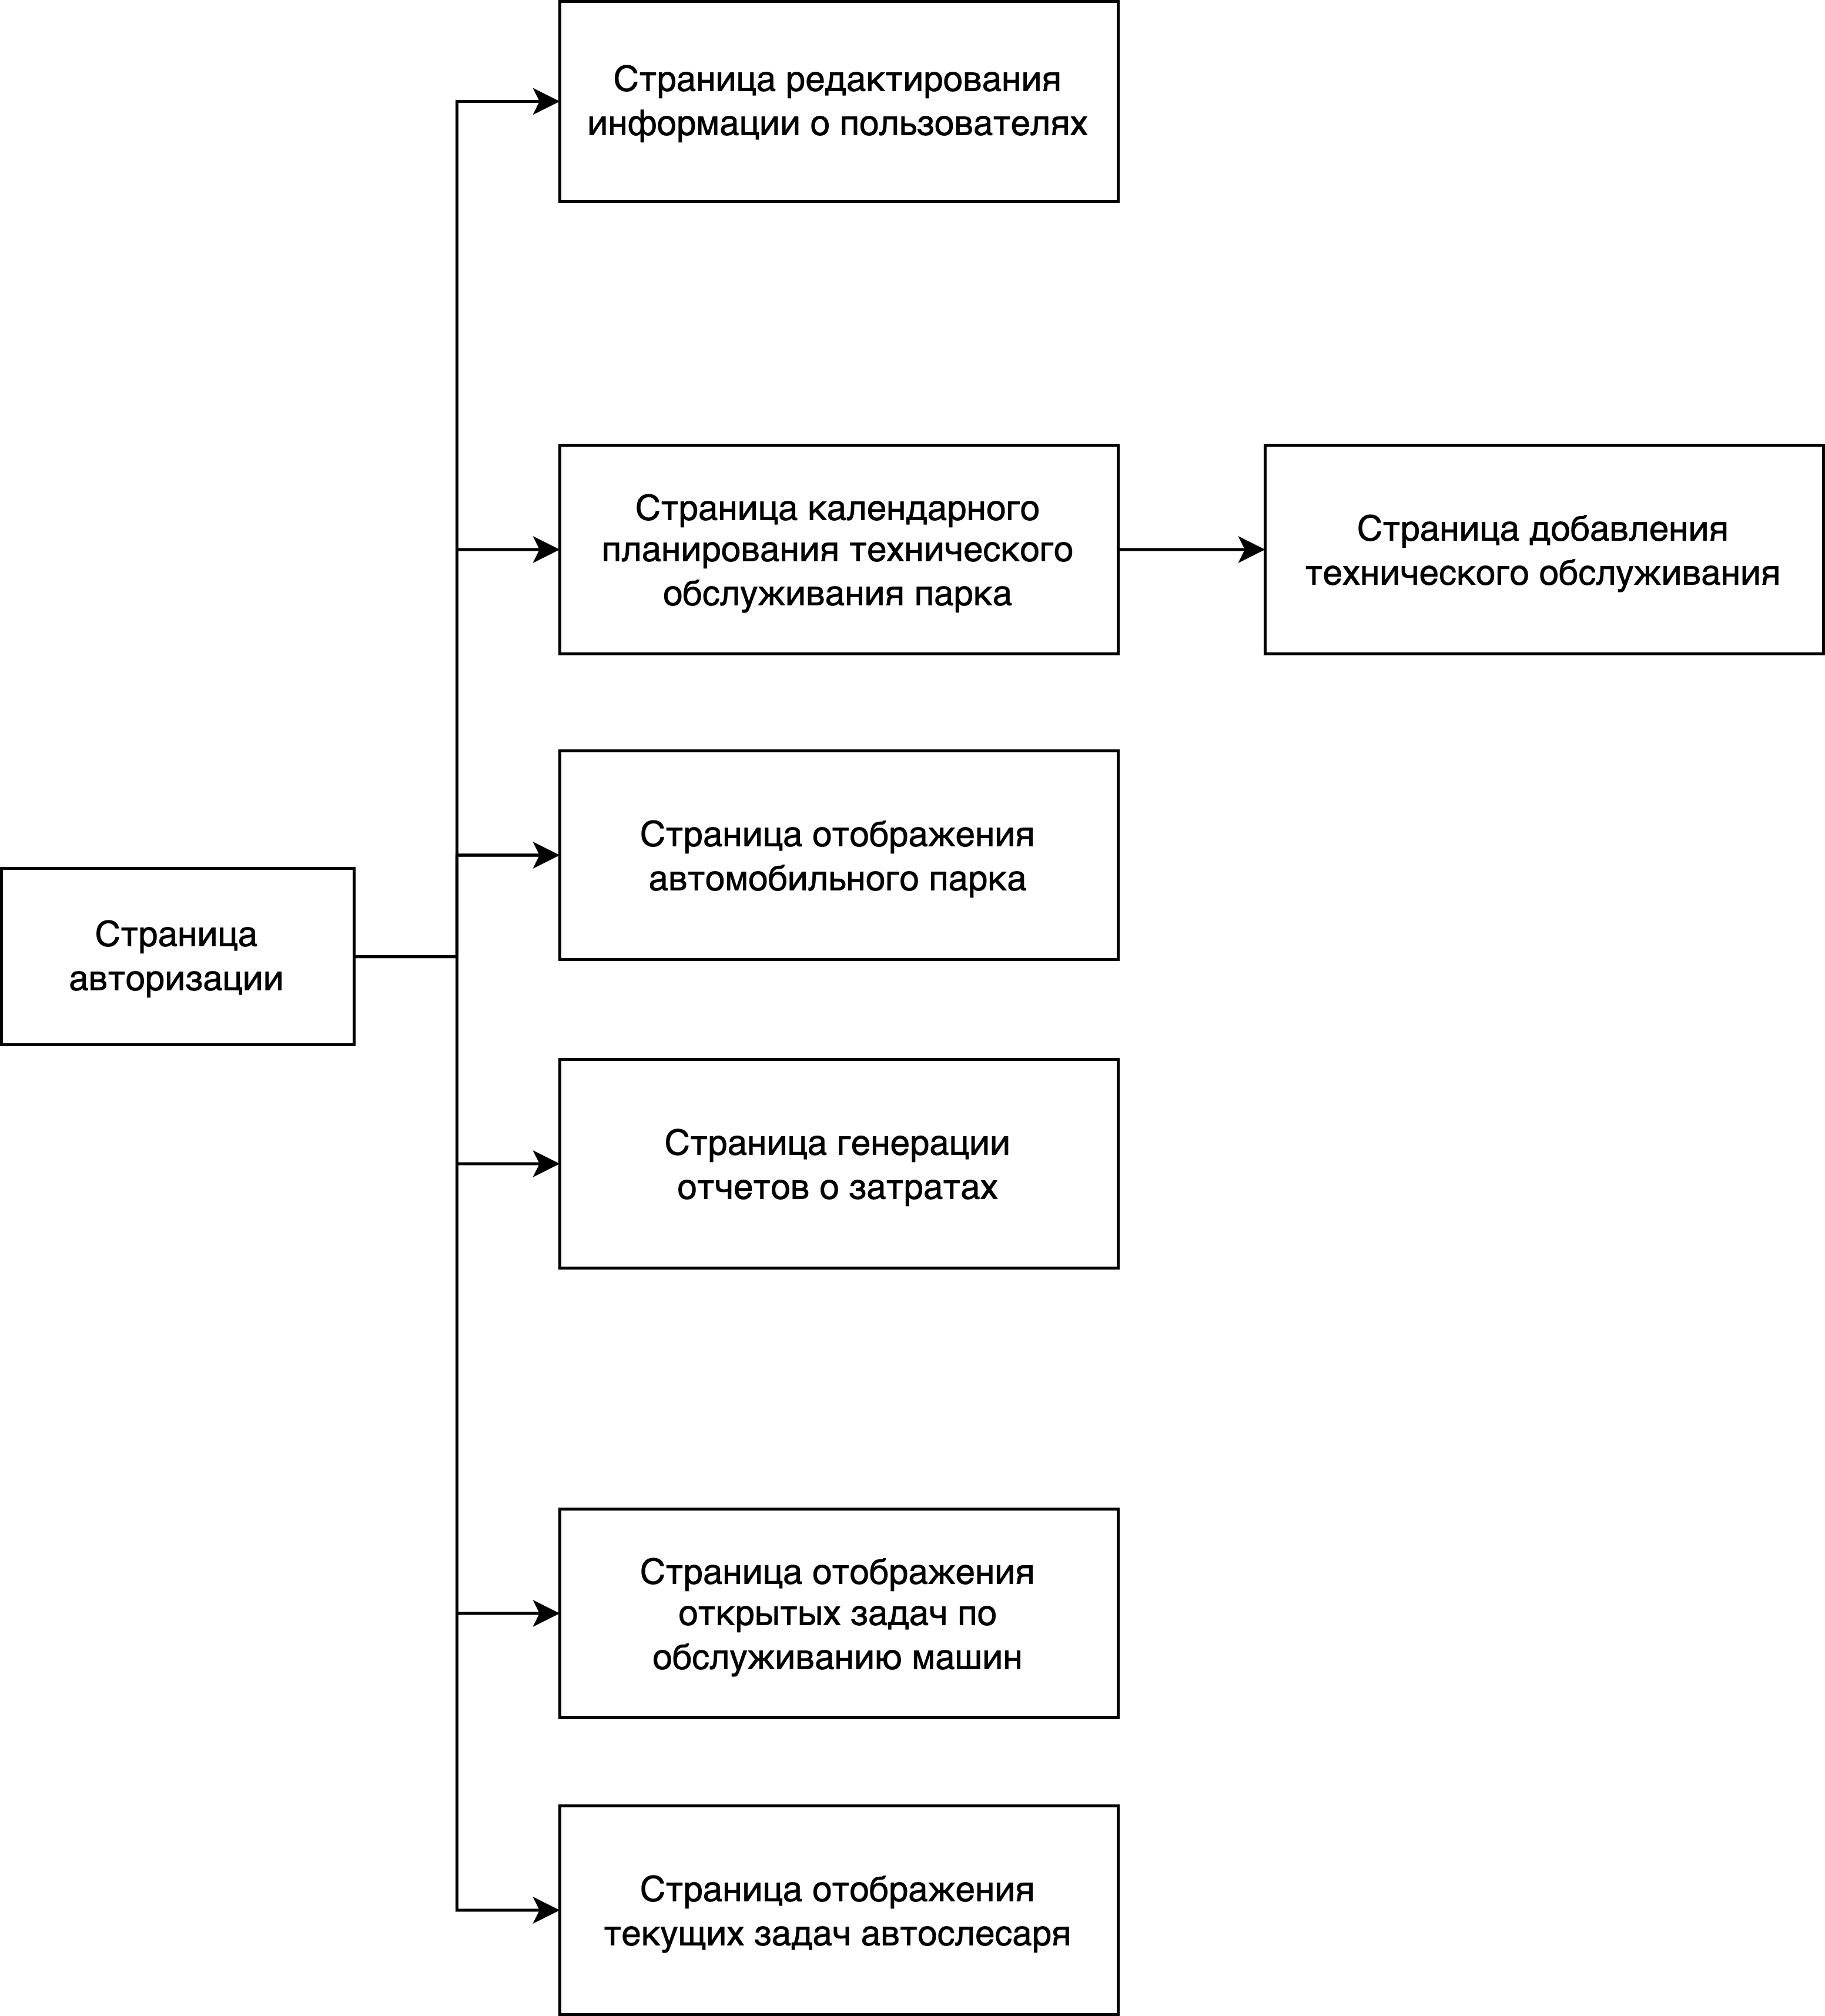
\includegraphics[width=\textwidth]{images/pages.png}
        \caption{Взаимодействие модулей системы друг с другом}
        \label{fig:pages}
    \end{figure}

    \subsubsection*{Используемые технические средства}

    Программа функционирует на двух системах: серверной и клиентской.

    На серверной части:

    В работе программы используются компьютеры на базе процессора x86, с
    поддержкой виртуализации, со стандартной конфигурацией и с установленной
    операционной системой, поддерживаемую Docker Engine.

    Для клиентской части:

    Клиентское приложение не зависит от архитектуры процессора и установленной ОС.
    Единственное требование -- современный веб-браузер с поддержкой исполнения
    Javascript на странице.

    \subsubsection*{Вызов и загрузка}

    Для запуска серверной части системы необходимо собрать образ
    Docker-контейнера. Необходимо скопировать файл
    \texttt{.env.example} в \texttt{.env} в корне проекта и изменить значения
    переменных окружения. После этого выполнить скрипт \texttt{deployment.sh},
    позволяющий автоматизировать сборку и запуск Docker-контейнера.

    После того, как серверное приложение запустится, необходимо настроить
    реверс-прокси Nginx, используя примерную конфигурацию, описанную в файле
    \texttt{nginx.conf}.

    \subsubsection*{Входные данные}
    Для администратора:
    \begin{enumerate}
        \item Данные для авторизации.
        \item Данные для регистрации новых пользователей.
    \end{enumerate}

    Для старшего техника:
    \begin{enumerate}
        \item Данные для авторизации.
        \item Данные для добавления нового технического обслуживания.
        \item Данные для регистрации нового автомобиля.
        \item Данные для генерации отчета.
    \end{enumerate}

    Для автослесаря:
    \begin{enumerate}
        \item Данные для авторизации.
        \item Данные о выполнении задач и технического обслуживания автомобиля.
    \end{enumerate}

    \subsubsection*{Выходные данные}
    Для старшего техника:
    \begin{enumerate}
        \item Календарный план проведения технического обслуживания парка
            автомобилей.
        \item Информация о парке автомобилей.
        \item Отчет о затратах за выбранный период времени.
    \end{enumerate}

    Для автослесаря:
    \begin{enumerate}
        \item Список доступных для выполнения задач по обслуживанию техники.
        \item Список текущих задач по обслуживанию конкретного автомобиля.
    \end{enumerate}

    \subsection{Описание применения программы}
    \subsubsection*{Назначение программы}

    Данная система предназначена для поддержки технического обслуживания
    автомобильного парка.

    Разработанное приложение позволяет просматривать календарное планирование
    технического обслуживания парка автомобилей, отслеживать текущий статус по
    выполнению задач обслуживания, генерировать отчеты о затратах при проведении
    работ на технике.

    \subsubsection*{Условия применения}

    Система состоит из двух модулей -- серверного и клиентского.

    Для серверного модуля необходимыми условиями являются наличие PostgreSQL
    версии 9 или выше, Docker Engine версии 20.10 или выше, веб-сервер Nginx
    версии 1.10 или выше.

    Для клиентского модуля необходим минимальный набор переферийных устройств,
    компьютер с современным браузером,
    поддерживающим стандарты HTML5, CSS3, а также с разрешением исполнения
    Javascript кода на странице.

    \subsubsection*{Описание задачи}

    Основной задачей системы является помощь в организации
    технического осмотра парка автомобилей

    \subsubsection*{Входные и выходные данные}
    Входные данные:

    Для администратора:
    \begin{enumerate}
        \item Данные для авторизации.
        \item Данные для регистрации новых пользователей.
    \end{enumerate}

    Для старшего техника:
    \begin{enumerate}
        \item Данные для авторизации.
        \item Данные для добавления нового технического обслуживания.
        \item Данные для регистрации нового автомобиля.
        \item Данные для генерации отчета.
    \end{enumerate}

    Для автослесаря:
    \begin{enumerate}
        \item Данные для авторизации.
        \item Данные о выполнении задач и технического обслуживания автомобиля.
    \end{enumerate}

    Выходные данные:

    Для старшего техника:
    \begin{enumerate}
        \item Календарный план проведения технического обслуживания парка
            автомобилей.
        \item Информация о парке автомобилей.
        \item Отчет о затратах за выбранный период времени.
    \end{enumerate}

    Для автослесаря:
    \begin{enumerate}
        \item Список доступных для выполнения задач по обслуживанию техники.
        \item Список текущих задач по обслуживанию конкретного автомобиля.
    \end{enumerate}

    \subsection{Описание результатов работы программы}

    В ходе работы было разработано приложение поддержки технического
    обслуживания автомобильного парка с удобным графическим
    интерфейсом. Использование технологии контейнеризации с использованием
    Docker позволяет с легкостью расширять систему, при необходимости увеличения
    производительности.

\end{document}
